\documentclass[DIN, pagenumber=false, fontsize=11pt, parskip=half]{scrartcl}

\usepackage{amsmath}
\usepackage{amsfonts}
\usepackage{amssymb}
\usepackage{enumitem}
\usepackage[utf8]{inputenc} % this is needed for umlauts
\usepackage[T1]{fontenc} 
\usepackage{commath}
\usepackage{xcolor}
\usepackage{booktabs}
\usepackage{float}
\usepackage{tikz-timing}
\usepackage{tikz}
\usepackage{multirow}
\usepackage{colortbl}
\usepackage{xstring}
\usepackage{circuitikz}
\usepackage{listings} % needed for the inclusion of source code
\usepackage[final]{pdfpages}
\usepackage{subcaption}
\usepackage{import}

\usetikzlibrary{calc,shapes.multipart,chains,arrows}

\newcommand{\Prb}[1]{P(\text{#1})}
\newcommand{\CPr}[2]{P(\text{#1}|\text{#2})}
\DeclareMathOperator*{\argmax}{arg\,max}
\DeclareMathOperator*{\argmin}{arg\,min}

%Inkscape fuckery
\newcommand{\incfig}[2][\columnwidth]{%
    \def\svgwidth{#1}
    \import{./}{#2.eps_tex}
}

\title{Pattern Recognition}
\author{Tim Luchterhand, Paul Nykiel, Jonas Strauch (Group P)}

\begin{document}
    \maketitle
    \section{Idea of Maximal Margin (SVM)}
    \begin{enumerate}
        \item
        The convex hulls of class $\omega_1$ and $\omega_{-1}$ are marked with a blue and an orange line respectively.
        \item
        The points with minimum distance on the convex hulls are marked in red.
        \item
        The line of maximum margin between $c_1$ and $c_{-1}$ is sketched in red.
        \item
        The separation line $s$ and the lines $l_1$ and $l_{-1}$ are labeled accordingly.
        \item
        The new points $x_1, x_2$ for class $\omega_1$ are drawn in blue and labeled accordingly. So are the points $x_3, x_4$
        for class $\omega_{-1}$, drawn in orange.
        \begin{figure}[h!]
            \centering
            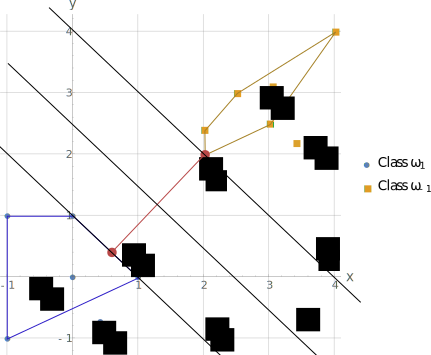
\includegraphics[scale=0.8]{a1.eps}
        \end{figure}
        \newpage
        \item
        Seperation line after point $x_5$ was added. 
        \begin{figure}[h!]
            \centering
            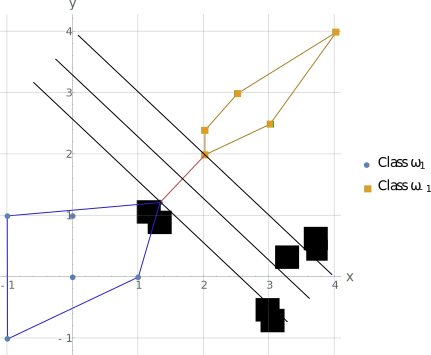
\includegraphics[scale=0.8]{a16.eps}
        \end{figure}
        \item
        Given the data is linear separable, the perceptron leanr algorithm find \textit{some} line which seperates both classes. The
        SVM finds \textit{the one line} which seperates both classes so that the minimum distance between both classes is maximized.
    \end{enumerate}

    \section{SVM}
    \begin{enumerate}
        \item
        \begin{align*}
        L(w, w_0, \alpha_1, \alpha_2) =& \sum_{i=1}^2{\alpha_i} - \frac{1}{2} \sum_{i=1}^2{\sum_{j=1}^2{\alpha_i \alpha_j T_i T_j \mathbf{x}_i^\text{T} \mathbf{x}_j}} \\
        \widehat{=}& \alpha_1 + \alpha_2 - \frac{1}{2}(2 \alpha_1^2 - 5 \alpha_1 \alpha_2 - 5 \alpha_2 \alpha_1 + 13 \alpha_2^2) \\
        =& \alpha_1 + \alpha_2 - \alpha_1^2 + 5 \alpha_1 \alpha_2 -\frac{13}{2} \alpha_2^2 \\
        \sum_{i=1}^2{\alpha_i T_i} =& \alpha_1 - \alpha_2 \stackrel{!}{=} 0
        \end{align*}

        \item
        \begin{align}
            \Lambda(\alpha_1, \alpha_2, \lambda) &= \alpha_1 + \alpha_2 - \alpha_1^2 + 5 \alpha_1 \alpha_2 -\frac{13}{2} \alpha_2^2 + \lambda (\alpha_1 - \alpha_2) \\
            \frac{\partial \Lambda}{\partial \alpha_1} &= 1 - 2 \alpha_1 + 5 \alpha_2 + \lambda \\
            \frac{\partial \Lambda}{\partial \alpha_2} &= 1 - 13 \alpha_2 + 5 \alpha_1 - \lambda \\
            \frac{\partial \Lambda}{\partial \lambda} &= \alpha_1 - \alpha_2 \\
            \nabla \Lambda &\stackrel{!}{=} \mathbf{0} \stackrel{(4)}{\Rightarrow} \alpha_1 = \alpha_2 \\
            (3) \stackrel{(5)}{\Rightarrow} \lambda &= 1 - 8 \alpha_1 \\
            (2) \stackrel{(7)}{\Rightarrow} \alpha_1 &= \alpha_2 = \frac{2}{5} 
        \end{align}
        \item
        \begin{align*}
            \mathbf{w} &= \sum_{i=1}^2{T_i \alpha_i \mathbf{x}_i} = \frac{2}{5} \begin{pmatrix} 1 \\ 1 \end{pmatrix} - \frac{2}{5} \begin{pmatrix} 2 \\ 3 \end{pmatrix} \\
            &= -\frac{2}{5} \begin{pmatrix} 1 \\ 2 \end{pmatrix} \\
            w_0 &= T_1 - \mathbf{w}^\text{T} \mathbf{x}_1 = 1 + \frac{6}{5} = \frac{11}{5}
        \end{align*}
        \newpage
        \item
        Resulting separation line.
        \begin{figure}[h!]
            \centering
            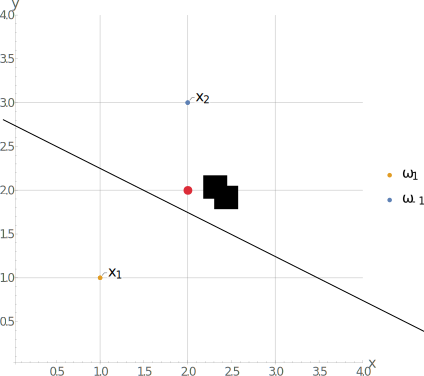
\includegraphics[scale=0.8]{a2.eps}
        \end{figure}
    \end{enumerate}
    
\end{document}
